\chapter{Estado del arte}
\label{chap:estado_arte}

Los fundamentos matemáticos y cuánticos presentados en el capítulo anterior constituyen todo el conocimiento necesario sobre el que se asienta el estado del arte de la representación vectorial de palabras. Representar el significado de una palabra mediante un vector numérico es el problema central que tanto Word2Vec como QWord2Vec buscan resolver, cada uno desde su propio paradigma computacional.

Este capítulo comienza con un repaso de toda la investigación realizada sobre los \textit{word embedding} así como las características que los definen, es decir, de qué modo la cercanía en el espacio vectorial codifica similitud semántica y por qué el espacio de Hilbert cuántico ofrece una alternativa estructuralmente afín al espacio euclídeo clásico. Sobre estos fundamentos, el capítulo siguiente describe en detalle los algoritmos Word2Vec y QWord2Vec, junto con las propuestas de mejora introducidas en este trabajo.

Los word embeddings son una de las técnicas más usadas en \gls{pln}. Gracias a los word embeddings, existen lenguajes de modelo como GPT-3, GPT-4, etc.

Estos algoritmos son rápidos y pueden generar secuencias de lenguaje y realizar otras tareas derivadas con alta precisión, incluyendo la comprensión contextual, propiedades semánticas y sintácticas, así como la relación lineal entre las palabras.

En esencia, estos modelos aprenden a extraer y representar patrones complejos a partir de secuencias de texto o voz, capturando tanto el significado como las relaciones entre las palabras. Pero, ¿cómo lo hacen?

En las siguientes secciones se explorará en mayor profundidad los word embeddings así como conceptos más avanzados de estos.

\section{Embeddings en Computación Clásica}
\label{sec:embeddings_clasicos}

\subsection{Evolución histórica de los \textit{word embeddings}}
\label{subsec:evolucion_historica}

La representación matemática y computacional del lenguaje natural ha sido uno de los desafíos más profundos en la historia del \gls{pln}. El desarrollo de los denominados \textit{word embeddings} (representaciones vectoriales de palabras) ha atravesado siete décadas de investigación, evolucionando a través de cuatro grandes paradigmas: métodos estadísticos, \textit{embeddings} estáticos, \textit{embeddings} contextuales y \textit{embeddings} de oraciones/documentos. Esta evolución demuestra una continua investigación y desarrollo en el que cada nueva técnica intentaba resolver las limitaciones semánticas, matemáticas y de escalabilidad de sus predecesoras, culminando en la actual era de los grandes modelos de lenguaje (\glsentryplural{llm}) \cite{nguyen_tracing_2026}.

\subsubsection{Representaciones estadísticas y modelos espaciales iniciales}

Los primeros intentos de representación textual se basaron fundamentalmente en la hipótesis distribucional formulada por Zellig Harris en 1954 \cite{harris_distributional_1954}, la cual postula que las palabras que ocurren en contextos similares tienden a poseer significados similares. En sus inicios, las arquitecturas utilizaban enfoques de \textit{one-hot encoding} \cite{salton_vector_1975}, donde cada palabra del vocabulario se representaba como un vector extremadamente extenso y disperso, compuesto íntegramente por ceros, a excepción de un único uno en la posición correspondiente al índice de la palabra. Aunque útil para crear índices, este método carecía de nociones de similitud semántica, ya que la distancia geométrica entre cualquier par de palabras era idéntica.

A partir de esta limitación, surgió el modelo \textit{Bag-of-Words} (BoW), que agregaba estos indicadores en un vector de frecuencia de términos para un documento completo. Sin embargo, seguían generándose vectores de muy alta dimensionalidad dominados por palabras muy frecuentes que aportaban poco valor semántico. Para solucionar esto, Karen Sparck Jones introdujo el concepto de TF-IDF (\textit{Term Frequency - Inverse Document Frequency}) \cite{jones_statistical_1972}. Este método preservaba la naturaleza dispersa del vector, pero introducía una métrica de informatividad: penalizaba las palabras omnipresentes y asignaba mayor peso a aquellos términos raros pero característicos de un documento. Se considera que el principio de asignar pesos variables según la relevancia en TF-IDF es un precursor conceptual del mecanismo de atención moderno.

Pese a esta mejora, los métodos basados en frecuencia no podían resolver la sinonimia ni la polisemia. El avance fundamental llegó con el Análisis Semántico Latente (LSA), propuesto por Deerwester et al. en 1990 \cite{deerwester_indexing_1990}. Mediante el uso de la descompocición en valores singulares (\gls{dvs}), el LSA lograba proyectar esa matriz dispersa hacia un espacio semántico latente de menor dimensión, agrupando conceptos afines. Finalmente, a principios de la década de los 2000, Bengio et al. \cite{bengio_neural_2003} desarrollaron el primer modelo de lenguaje probabilístico neuronal, demostrando que era posible aprender representaciones densas optimizando una red neuronal para predecir la siguiente palabra mediante propagación hacia atrás (\textit{backpropagation}), sentando las bases absolutas para los \textit{embeddings} modernos.

\subsubsection{La revolución de los \textit{embeddings} de palabras estáticos}

El gran salto hacia el uso masivo de vectores densos ocurrió en 2013 con la introducción de Word2Vec por Tomas Mikolov y su equipo \cite{mikolov_efficient_2013}. Word2Vec propuso dos arquitecturas predictivas altamente eficientes: \textit{Continuous Bag-of-Words} (CBOW), que predecía una palabra objetivo a partir de su contexto, y \textit{Skip-Gram}, que utilizaba la palabra objetivo para predecir el contexto. Este modelo logró traducir relaciones semánticas y sintácticas en operaciones algebraicas simples (como la capacidad de resolver la analogía $\vec{v}(\text{Rey}) - \vec{v}(\text{Hombre}) + \vec{v}(\text{Mujer}) \approx \vec{v}(\text{Reina})$). No obstante, dependía de ventanas de contexto locales pequeñas y no utilizaba eficientemente la información global del corpus.

Para subsanar esta debilidad, Pennington et al. desarrollaron GloVe (\textit{Global Vectors}) en 2014 \cite{pennington_glove_2014}. GloVe funcionaba factorizando explícitamente una matriz global de coocurrencia palabra-contexto utilizando mínimos cuadrados ponderados. Esto resultó en un espacio vectorial mucho más estable, combinando las ventajas del conteo estadístico con las representaciones neuronales. Paralelamente, investigadores como Levy y Goldberg (2014) \cite{levy_dependency_2014} cuestionaron el uso de ventanas de proximidad lineal y propusieron \textit{embeddings} basados en dependencias sintácticas. Esto permitió agrupar las palabras por su rol funcional en la oración en lugar de su parentesco temático (por ejemplo, agrupar escuelas diferentes entre sí en lugar de asociar una escuela a sus alumnos).

El límite práctico de Word2Vec y GloVe era el manejo de palabras fuera del vocabulario y la morfología compleja. FastText, presentado por Bojanowski et al. en 2017 \cite{bojanowski_enriching_2017}, resolvió esto representando cada palabra como una bolsa de n-gramas de caracteres (subpalabras). Esto permitió al modelo componer vectores significativos para palabras nunca antes vistas sumando los vectores de sus fragmentos. Sin embargo, todos estos modelos compartían un defecto insalvable: eran estáticos. Asignaban un único vector fijo a cada palabra, colapsando todos sus significados posibles en uno solo. Aunque intentos como Sense2Vec (Trask et al., 2015) \cite{trask_sense2vec_2015} intentaron paliar esto etiquetando las palabras con su categoría gramatical (separando el sustantivo del verbo), la solución definitiva requería un cambio de paradigma.

\subsubsection{Embeddings contextuales y la transición a arquitecturas dinámicas}

La incapacidad de manejar la polisemia impulsó la adopción de \textit{embeddings} contextuales, un cambio catalizado por la arquitectura \textit{Transformer} introducida por Vaswani et al. en 2017 \cite{vaswani_attention_2017}. El \textit{Transformer} introdujo el mecanismo de autoatención (\textit{self-attention}), permitiendo procesar el contexto global de una secuencia en paralelo y calcular dinámicamente cómo cada palabra afectaba a las demás, rompiendo el cuello de botella secuencial de las redes recurrentes.

Antes del dominio total del \textit{Transformer}, el modelo ELMo propuesto por Peters et al. en 2018 \cite{peters_deep_2018} demostró que se podían generar vectores distintos para la misma palabra según su oración utilizando redes neuronales recurrentes bidireccionales (Bi-LSTM). ELMo generaba representaciones jerárquicas donde las capas bajas captaban la sintaxis y las altas la semántica.

El impacto definitivo lo marcó BERT, lanzado por Devlin et al. en 2019 \cite{devlin_bert_2019}. BERT utilizó el codificador del \textit{Transformer} preentrenado mediante el modelado de lenguaje enmascarado (MLM) y la predicción de la siguiente oración (NSP). Esto le otorgó una comprensión bidireccional que revolucionó las tareas de comprensión lectora. Simultáneamente, la familia de modelos GPT de Radford et al. \cite{radford_improving_2018} utilizó el decodificador del \textit{Transformer} con un enfoque autorregresivo unidireccional, entrenándose para predecir la siguiente palabra, lo que sentó las bases para la generación de texto a largo plazo y el razonamiento generativo.

\subsubsection{Embeddings de frases, documentos y la recuperación semántica}

Históricamente, fue necesario codificar secuencias completas más allá de palabras individuales. Le y Mikolov adaptaron su propio trabajo en 2014 para crear Doc2Vec \cite{le_distributed_2014}, introduciendo un vector de párrafo que actuaba como una memoria temática del documento. Posteriormente, Kiros et al. (2015) \cite{kiros_skip_2015} propusieron los \textit{Skip-Thought Vectors}, que aplicaban el objetivo de \textit{Skip-Gram} a nivel de oración, obligando al modelo a predecir las oraciones circundantes para capturar propiedades discursivas.

Para proporcionar un estándar universal y eficiente, Cer et al. introdujeron el \textit{Universal Sentence Encoder} (USE) en 2018 \cite{cer_universal_2018}, entrenado en múltiples tareas para lograr una generalización masiva. No obstante, el avance más transformador en este subcampo fue Sentence-BERT (S-BERT), propuesto por Reimers y Gurevych en 2019 \cite{reimers_sentence_2019}. Al notar que el vector nativo de BERT era deficiente para comparar similitudes, adaptaron la arquitectura utilizando redes siamesas. Esto redujo el tiempo necesario para buscar oraciones similares en corpus masivos de horas a solo milisegundos, impulsando los sistemas de búsqueda semántica modernos.

\subsubsection{El impacto de GPT-3 y la era de los LLMs (2020 - Actualidad)}

La investigación en \textit{word embeddings} experimentó una disrupción estructural con el lanzamiento de GPT-3 por Brown et al. en 2020 \cite{brown_language_2020}. Con 175 mil millones de parámetros, demostró que los \textit{embeddings} ya no necesitaban ser componentes aislados. A partir de este momento, la producción de artículos centrados exclusivamente en \textit{embeddings} estáticos o estadísticos se desplomó. Los \textit{embeddings} han pasado a subsumirse como capas de representación internas dentro de inmensos modelos de aprendizaje profundo de extremo a extremo (\textit{end-to-end}).

Esta última transición ha provocado que el campo se desplace de pequeños grupos de investigación académica a grandes consorcios corporativos, debido a los inmensos recursos computacionales requeridos. Sin embargo, la investigación contemporánea no ha abandonado las teorías previas; al contrario, métodos clásicos de frecuencia siguen integrándose hoy en arquitecturas híbridas (como la generación aumentada por recuperación o RAG) para complementar a las redes neuronales, demostrando que las siete décadas de innovación en representación textual mantienen una profunda continuidad histórica.

\subsection{Introducción al concepto de \textit{Embedding}}
\label{sec:introduccion_embedding}

De manera intuitiva, un \textit{embedding} de texto es una representación matemática que proyecta un fragmento de texto en un espacio latente de alta dimensionalidad. En este espacio, la posición del texto se define mediante un vector, donde cada componente del vector corresponde a una dimensión. Al igual que en un plano cartesiano se tienen dos dimensiones, en un embedding, se suele trabajar con muchas más dimensiones para representar una palabra en el espacio\cite{henner_intuitive_embeddings_2023}. Por ejemplo, el modelo de \textbf{OpenAI} \textit{text-embedding-ada-002} el cual tiene un espacio de dimensión de 1536. Es decir, cada vector está formado por 1536 componentes.

Un ejemplo de cómo se verían los valores que toma cada dimensión es el siguiente:

\begin{quote}
  \textit{``A text embedding is a piece of text projected into a high-dimensional latent space. The position of our text in this space is a vector, a long sequence of numbers. Think of the two-dimensional cartesian coordinates from algebra class, but with more dimensions---often 768 or 1536.''} \cite{henner_intuitive_embeddings_2023}
\end{quote}

Al procesar el párrafo anterior mediante el modelo \textit{text-embedding-ada-002} mencionado, se obtiene la gráfica de la Figura \ref{fig:ejemploValoresEmbedding}, donde cada barra vertical representa el valor asignado a una de sus 1536 dimensiones.

\begin{figure}[h]
  \centering
  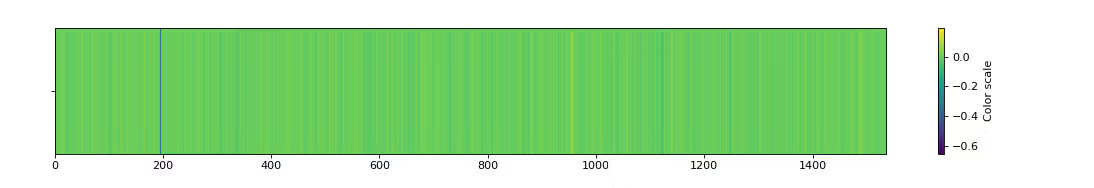
\includegraphics[width=1.2\linewidth]{imagenes/ejemploValoresEmbedding.png}
  \caption{Representación gráfica de los valores en las 1536 dimensiones de un embedding generado por el modelo text-embedding-ada-002. Fuente: \cite{henner_intuitive_embeddings_2023}.}
  \label{fig:ejemploValoresEmbedding}
\end{figure}

Un \textbf{espacio de embedding} o \textbf{espacio latente} se define matemáticamente como un espacio donde los elementos están posicionados de manera más cercana uno del otro cuando tienen valores parecidos, mientras que si difieren dichos elementos, se posicionan más lejos entre ellos. En el caso del \gls{pln}, frases que son semánticamente más similares a otras tendrán un vector de embedding similar, por lo que estarán más juntas en el espacio.

Aunque la comparación entre frases es una de las aplicaciones más conocidas, los \textit{embeddings} también se aplican en modelos de \gls{ml} y en arquitecturas de redes neuronales complejas.

\subsubsection{Embeddings de palabras (\textit{Word Embeddings})}

Mientras que el concepto general de \textit{embedding} puede aplicarse a frases completas (como en el ejemplo introducido), su uso más extendido e histórico se encuentra en su aplicación a nivel atómico: las palabras. Un \textit{embedding} de palabras, es un vector de longitud fija el cual su único cometido, es representar una única palabra o \textit{token} \cite{almeida_word_2023}.

El diseño y creación de estos vectores se clasifica principalmente en dos grandes familias estratégicas, dependientes de sus algoritmos de generación: los \textbf{modelos basados en predicciones} y los \textbf{modelos basados en conteos}.

\paragraph{Modelos basados en predicciones}

Esta técnica de representación surgió fuertemente ligada al desarrollo de los \gls{mnl}. A diferencia de los enfoques estadísticos tradicionales de recuento, un modelo predictivo se centra en aprender el significado de un término de forma prospectiva, es decir, ``adivinando''.

Para lograrlo, emplean una red neuronal sencilla dotada de una ventana de contexto de tamaño fijo y móvil (por ejemplo, avanzando de cinco en cinco palabras). A medida que lee el texto, el modelo intenta predecir el significado de una palabra central en base a las palabras vecinas de esta ventana, o a la inversa, predecir el contexto apoyándose únicamente en dicho término central.

El aspecto fundamental en todo esto, es que tras finalizar el entrenamiento, el objetivo de \gls{ml} deja de ser la capacidad del modelo para adivinar con exactitud. En su lugar, de la red neuronal, se extraen los \textbf{pesos y valores} que ha ajustado internamente. Estos valores que fueron ajustados durante el entrenamiento se convierten directamente en el \textit{word embedding}. En consecuencia, el mecanismo iterativo garantiza que aquellas palabras empleadas en contextos idénticos acaben reteniendo representaciones vectoriales prácticamente iguales, tal y como se muestra en la Figura \ref{fig:word_embeddings_model}.

\begin{figure}[h]
  \centering
  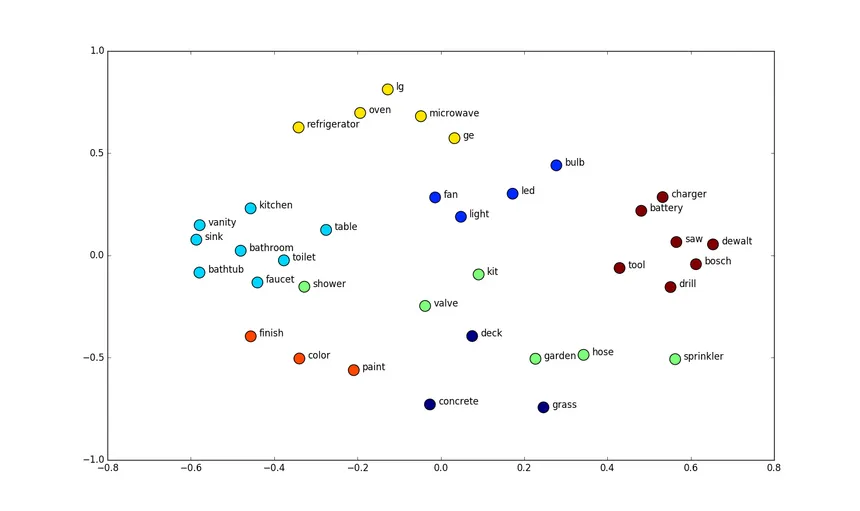
\includegraphics[width=1.0\linewidth]{imagenes/Word-embeddings-model.png}
  \caption{Representación visual de un modelo basado en predicciones para generar embeddings de palabras. Fuente: \cite{neptune_word_embeddings_guide}.}
  \label{fig:word_embeddings_model}
\end{figure}

Una de las arquitecturas más representativas dentro de la predicción de \textit{embeddings} es la famosa familia algorítmica \textbf{Word2Vec}, en concreto \textbf{SkipGram} que se detalla de forma exhaustiva en el próximo capítulo.

\paragraph{Modelos basados en conteos}

Por su parte, la segunda categoría de modelos hace uso de la estadística global a lo largo de un documento completo (\textit{corpus}). Estos modelos se aprovechan de los recuentos de coocurrencia (palabra y contexto) estructurando toda la información como grandes \textit{matrices de palabra-contexto}.

El funcionamiento radica en la creación de una matriz gigantesca donde se contabiliza el número de apariciones conjuntas en las que una palabra acompaña a todo un posible contexto del propio texto. No obstante, si el conjunto de datos cuenta con $n$ palabras distintas, las dimensiones de la matriz ascenderán a un total de $n \times n$. Esto acarrea severamente un cuello de botella de almacenamiento. Adicionalmente, la inmensa mayoría de cruces de dicha matriz representarán palabras que jamás han coexistido en el texto (por ejemplo, ``oveja'' y ``pantalla''), llenando de ceros el modelo de datos. Esta estructura tan ineficiente es conocida como \textbf{matriz dispersa}.

Para solventar esta carencia y la falta de memoria, se reduce la dimensionalidad a través de complejas operaciones de álgebra lineal, como puede ser la \gls{dvs}. Con esto logran sintetizar enormes matrices de ceros, transformándolos en \textbf{vectores cortos y densos}. De tal modo, que los conceptos globalmente equivalentes retengan valores numéricamente similares sin desperdiciar memoria.

La \textbf{mayor ventaja} de esta táctica estadística contable, frente al sistema predictivo, reside precisamente en que es capaz de aprovechar la información global de todo el \textit{corpus}, un aspecto estadístico que se le escapa a las ventanas de lectura en las redes neuronales por definición.

El modelo híbrido con más popularidad en este ámbito es el de \textbf{GloVe (\textit{Global Vectors})} \cite{pennington_glove_stanford}. Desarrollado por un equipo de investigadores de la Universidad de Stanford, logra exitosamente agrupar los beneficios numéricos de las matrices grandes de conteo global, con las altas capacidades de optimización paramétrica propias de los modelos del \gls{ml}, como se ilustra en la Figura \ref{fig:word_embedding_counting_model}.

\begin{figure}[h]
  \centering
  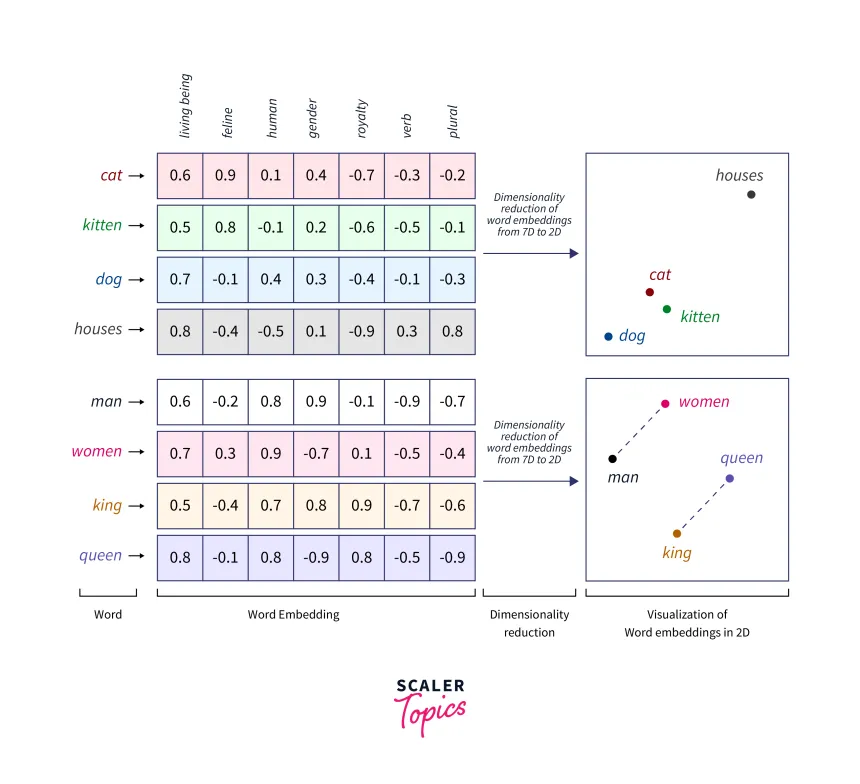
\includegraphics[width=0.9\linewidth]{imagenes/word-embedding-counting-model.png}
  \caption{Representación visual de un modelo basado en conteos para generar embeddings de palabras. Fuente: \cite{malingan_tensorflow_embeddings_2023}.}
  \label{fig:word_embedding_counting_model}
\end{figure}

\subsection{Mecanismos geométricos de los embeddings}

Una vez comprendido que un embedding proyecta palabras en un espacio continuo donde la cercanía espacial equivale a similitud semántica, surgen dos interrogantes fundamentales en el diseño de estos sistemas: ¿cómo se estructuran los ejes de este espacio para encapsular el significado complejo del lenguaje? y ¿cómo se calcula con precisión matemática la distancia entre dos vectores?

Para responder a la primera cuestión, es necesario analizar el papel de la \textbf{información latente} \cite{henner_intuitive_embeddings_2023}, la cual permite pasar de representaciones dispersas a vectores densos basados en atributos ocultos. Para la segunda, se debe explorar \textbf{métricas de distancia} específicas que sean efectivas en espacios de tantas dimensiones.

\subsubsection{Métricas de Distancia}

Como se explicó con anterioridad, una de las características principales de un embedding representado en el espacio, es que mantiene la distancia. Los vectores de alta dimensionalidad que se utilizan en los embeddings de palabra (así como en los \glsentryplural{llm}), no son intuitivos. Pero la intuición espacial se mantiene igual mientras reducimos la escala de estos.

Un ejemplo básico es el siguiente: imagina un plano de planta bidimensional de una biblioteca de una sola planta. Los usuarios de la biblioteca son amantes de los gatos, de los perros, o se sitúan en algún punto intermedio. El objetivo es colocar los libros sobre gatos cerca de otros libros de gatos, y los libros sobre perros cerca de otros libros de perros.

El enfoque más sencillo se conoce como el modelo de bolsa de palabras. Consiste en establecer un eje de perros a lo largo de una pared y un eje de gatos perpendicular a él. A continuación, se cuentan las ocurrencias de las palabras ``gato'' y ``perro'' en cada libro y se ubica dicho libro en su punto correspondiente dentro del sistema de coordenadas $(\text{perro}_x, \text{gato}_y)$.

Pensemos ahora en un sistema de recomendación sencillo. A partir de la selección anterior de un libro, ¿qué se podría sugerir a continuación? Bajo la suposición (muy simplificada) de que estas dos dimensiones capturan adecuadamente las preferencias del lector, basta con buscar el libro que se encuentre más cerca. En este caso, el sentido intuitivo de cercanía es la distancia euclídea —el camino más corto entre dos libros—:

\[
  d(\mathbf{p}, \mathbf{q}) = \sqrt{\sum_{i=1}^{n} (q_i - p_i)^2};
\]

Siguiendo el razonamiento lógico, si se analiza a través de la distancia euclídea, se pondrá el libro $(\text{perro}_5, \text{gato}_1)$ más cerca del libro $(\text{perro}_1, \text{gato}_5)$ que de un libro mucho más extenso o enciclopédico como $(\text{perro}_{100}, \text{gato}_1)$. Esto plantea un grave problema semántico: un lector de libros cortos de perros con proporción $(5, 1)$ seguramente prefiera a continuación una enciclopedia gigante sobre perros de $(100, 1)$ antes que un libro corto sobre gatos de $(1, 5)$. La métrica euclídea penaliza severamente la longitud en palabras del libro (magnitud) omitiendo por completo el reparto del tema de este (la proporción).

Cuando resulta más relevante concentrarse en los pesos relativos temáticos que en sus magnitudes absolutas, los vectores se normalizan. Esto se logra dividiendo en ambos la cantidad de apariciones de perros y gatos para obtener la conocida \textbf{similitud coseno} \cite{porter_understanding_2023}. De manera más visual, este cálculo equivale geométricamente a proyectar todos los puntos disponibles en el espacio sobre una circunferencia de radio unidad (es decir, que el módulo de todos los vectores es $1$) y medir la distancia a lo largo del arco que los une. Al ignorar la longitud del documento original, se evalúa únicamente la dirección del vector respecto al origen, logrando una métrica de similitud mucho más robusta y natural al lenguaje humano.

Matemáticamente, esta métrica se define mediante el cociente del producto escalar de dos determinados vectores entre el producto de sus magnitudes:

\[
  \text{similitud}(\mathbf{p}, \mathbf{q}) = \cos(\theta) = \frac{\mathbf{p} \cdot \mathbf{q}}{\|\mathbf{p}\| \|\mathbf{q}\|} = \frac{\sum_{i=1}^{n} p_i q_i}{\sqrt{\sum_{i=1}^{n} p_i^2} \sqrt{\sum_{i=1}^{n} q_i^2}};
\]

Un pensamiento intuitivo para entender la fórmula de similitud coseno, es que si dos vectores apuntan en la misma dirección, el ángulo entre ellos es 0 por lo que le coseno es 1. Si son ortogonales, significa que no comparten una 'direccionalidad', el coseno es 0.

En el contexto que nos encontramos de embeddings de palabras, hay que pensar que cada vector actúa como una flecha que apunta desde el origen hasta la posición de la palabra en nuestra librería imaginada. Palabras que son similares semánticamente tendrán vectores que apuntan en direcciones similares, es decir, la similitud coseno será mayor, tal y como se puede apreciar gráficamente en la Figura \ref{fig:ejemploSimilitudCoseno}.

\begin{figure}[h]
  \centering
  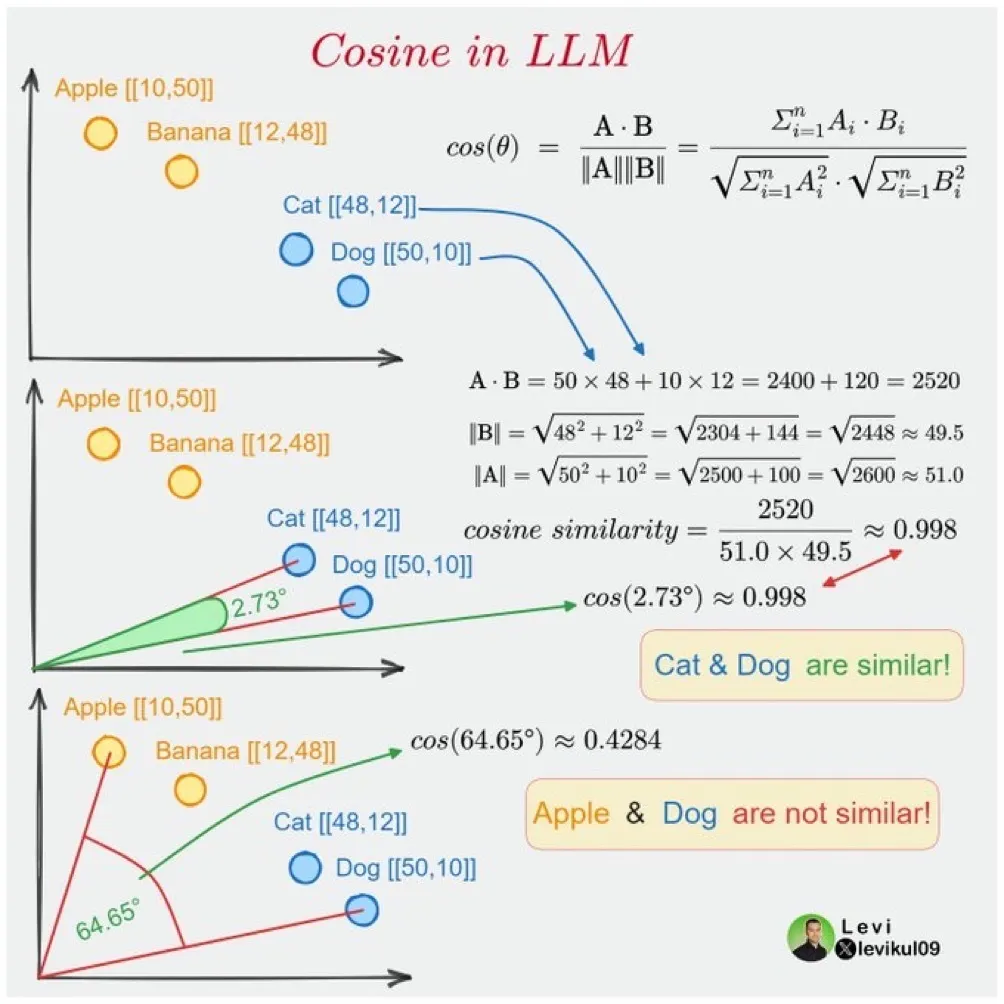
\includegraphics[width=0.7\linewidth]{imagenes/ejemploSimilitudCoseno.png}
  \caption{Ejemplo visual de la representación de vectores y su cercanía empleando la similitud coseno. Fuente: \cite{levikul09_cosine_similarity_x}.}
  \label{fig:ejemploSimilitudCoseno}
\end{figure}

\subsubsection{Información Latente}

Cualquier texto suele emplear sinónimos o términos relacionados para referirse a un mismo concepto; por ejemplo, volviendo al mismo ejemplo de antes, un libro sobre perros utilizará frecuentemente palabras como ``canino''. En un modelo básico de bolsa de palabras, incorporar este nuevo vocablo requiere añadir una dimensión perpendicular adicional a las ya existentes, transformando nuestro anterior sistema de coordenadas en $(\text{perro}_x, \text{gato}_y, \text{canino}_z)$.

Bajo este mismo principio, resulta muy sencillo continuar agregando nuevas dimensiones para representar más palabras, consiguiendo un espacio multidimensional $(\text{perro}_x, \text{gato}_y, \text{canino}_z, \text{felino}_w)$. Sin embargo, este enfoque tan básico conlleva dos grandes problemas que imposibilitan su aplicación a gran escala: rompe de inmediato la interpretabilidad espacial (como lo era la sencilla idea inicial de una biblioteca bidimensional) y provoca una explosión en los requisitos necesarios para el cómputo.

Resulta evidente que, a nivel computacional, esta aproximación es extremadamente ineficiente a medida que aumenta el tamaño del vocabulario. El español, por ejemplo, cuenta con más de 93.000 palabras según el Diccionario de la Real Academia Española \cite{espanol_palabras_2022}. Manejar vectores con decenas de miles de dimensiones implica calcular una ingente cantidad de combinatorias. Además, se agrava el problema de la dispersión de datos: en un documento dado, la gran mayoría del vocabulario total no aparecerá, rellenando los vectores con innumerables ceros que penalizan drásticamente el rendimiento de los modelos estadísticos y de aprendizaje automático.

La solución a la alta dimensionalidad radica en abstraer el conteo literal hacia ejes que representen verdaderos atributos semánticos. Si el modelo es capaz de identificar la relación semántica entre ``gato'' y ``felino'', podría agrupar la contribución de ambas en una única variable latente compartida. Esto no solo comprime el tamaño de los vectores, haciendo a los algoritmos mucho más eficientes y veloces, sino que también genera una representación geométrica mucho más afín a la intuición humana.

De la misma forma, términos más amplios como ``mascota'' o ``mamífero'' representan características semánticas compartidas simultáneamente por ``perro'' y ``gato''. En un espacio latente bien optimizado, estas palabras genéricas actúan como atributos comunes que vinculan y aproximan ambos animales en ciertas dimensiones del espacio. Por otro lado, si la elevada reducción dimensional provocara una superposición excesiva donde términos que debieran ser distintos terminen colapsando —por ejemplo, confundiéndose ambos en el mismo punto exacto—, esta carencia de precisión podría mitigarse introduciendo nuevos ejes latentes. Estos nuevos atributos ocultos de diferenciación (por ejemplo, proyectando qué palabras se relacionan estrechamente con ``mesa'' frente a los animales vivos mencionados anteriormente) permiten desenredar los agrupamientos de datos semánticos complejos.


\section{Embeddings en Computación Cuántica}
\label{sec:embeddings_cuanticos}

El procesamiento de lenguaje natural ha comenzado a explorar el paradigma cuántico como una alternativa para superar las limitaciones de espacio y expresividad de los modelos clásicos. En esta sección se aborda la fundamentación teórica que justifica la representación de conceptos lingüísticos dentro de espacios vectoriales cuánticos.

\subsection{Paralelismo entre Espacio Semántico y Espacio de Hilbert}

Como se vio en capítulos anteriores, los estados en computación cuántica están representados por vectores definidos en un espacio complejo, el cual se conoce formalmente como \textbf{espacio de Hilbert} ($\mathcal{H}$) \cite{quandela_hilbert_space}. Por su parte, en el \gls{pln} clásico se modela el significado de las palabras mapeándolas a vectores en un espacio vectorial puramente real ($\mathbb{R}^n$).

A partir de esta analogía natural, surge la posibilidad de modelar las palabras y sus significados como estados dentro del propio espacio de Hilbert \cite{wittek_combining_semantics}.

\subsubsection{Codificación multidimensional: Forma y Contenido}

En un espacio semántico tradicional, el significado de una palabra adquiere ``sustancia'' al ubicarse en unas coordenadas determinadas que definen su forma. Sin embargo, al restringirse al uso exclusivo de los números reales, el \gls{pln} clásico queda comúnmente limitado a capturar únicamente su \textit{semántica distribucional} (las estadísticas y frecuencias con las que coocurre junto a otras palabras).

Al trasladar el procesamiento de lenguaje al dominio cuántico de Hilbert, las propiedades exclusivas de los números complejos permiten unificar distintos niveles de información semántica en un único vector de estado. Esto logra vincular el uso externo del lenguaje (su \textit{forma}) directamente con su fundamento conceptual intrínseco (su \textit{contenido}). Para ello, se propone una división explícita de las dimensiones de almacenamiento:

\begin{itemize}
  \item \textbf{Componente Real:} Se utiliza de la misma forma para codificar la \textit{semántica distribucional}. Captura el uso estadístico clásico, determinando el comportamiento de la palabra estrictamente en base a su contexto y al número de interacciones o apariciones que realiza con respecto a las palabras que le rodean en los distintos documentos analizados.
  \item \textbf{Componente Imaginaria:} Se reserva de forma ortogonal para alojar la \textit{semántica referencial u ontológica}. Representa los fundamentos preexistentes, los conceptos formales o el núcleo estricto que designa la propia palabra (el significado que podría extraerse de ontologías taxonómicas u organizaciones como base de conocimientos, por ejemplo \textit{WordNet} o diagramas \textit{SNOMED-CT}).
\end{itemize}

Esta división entre semántica distribucional y referencial, y cómo ambas conviven en el mismo espacio vectorial complejo, queda representada esquemáticamente en la Figura \ref{fig:componentesEmbeddingsCuanticos}.

\begin{figure}[h]
  \centering
  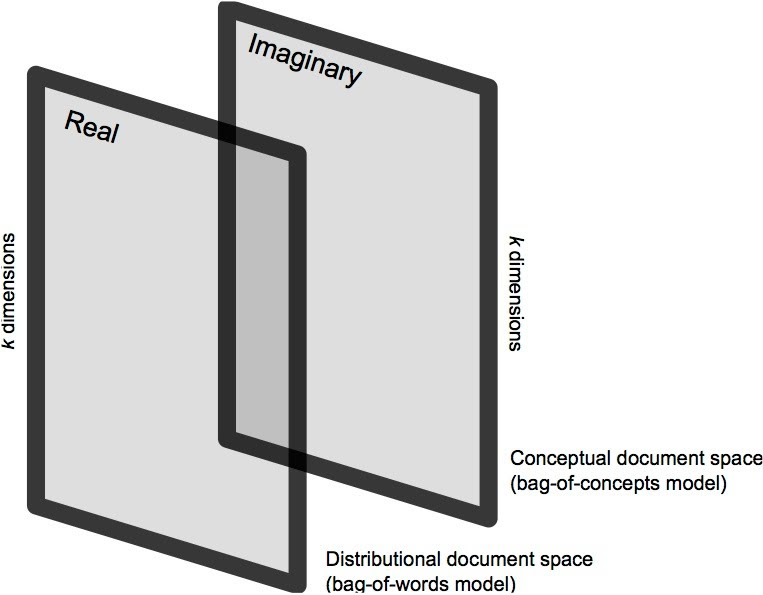
\includegraphics[width=0.5\linewidth]{imagenes/componentesEmbeddingsCuanticos.jpg}
  \caption{Esquema del espacio documental complejo vectorial unificando la semántica distribucional y referencial en el espacio de Hilbert. Fuente: \cite{wittek_combining_semantics}.}
  \label{fig:componentesEmbeddingsCuanticos}
\end{figure}

\subsubsection{Afinidad Cuántica, Superposiciones y Fases}

En el apartado clásico se demostró que la afinidad semántica puede medirse mediante distintas distancias sobre un espacio real continuo. No obstante, al emplear el espacio de Hilbert esta medición no solo relaciona dos palabras distintas, sino que va un paso más allá. Al tratar con números complejos, es posible medir la distancia cuantitativa que existe entre la parte estadística de uso de la palabra (su componente real) y su definición conceptual referencial alojada en su componente imaginaria.

Para este análisis se evalúa la \textbf{fase o ángulo} que se forma interactivamente entre ambas componentes, logrando que el producto interno refleje tanto la componente real como imaginaria del contenido.



Descritas las propiedades geométricas y semánticas que fundamentan las representaciones vectoriales de palabras, el capítulo siguiente presenta los dos algoritmos centrales de este trabajo ---Word2Vec y QWord2Vec--- junto con las propuestas de mejora introducidas sobre el modelo cuántico original.

